\documentclass{article}
\usepackage{tikz, comment}
\usepackage{pifont}
\usepackage{fontspec}
\usetikzlibrary{arrows, decorations.markings, decorations.pathreplacing}
\begin{comment}
:Title: Not defined yet
:Slug: No name yet

Description Here.........
\end{comment}
\begin{document}\centering 

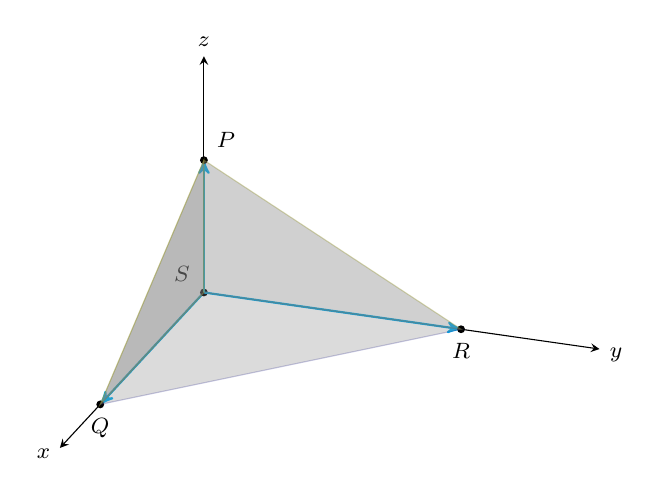
\begin{tikzpicture}[font=\footnotesize]
\pgfplotsset{compat=1.8}
\begin{axis}
[axis lines = center, view={110}{35}, scale=1., ticks=none, 
axis background, xlabel = {$x$}, ylabel ={$y$}, zlabel ={$z$}, domain =0:1, y domain =0:1,
xmin =0,
xmax =2.5,
ymin =0,
ymax =2,
zmin =0, 
zmax =2.5,
%samples =10, samples y =40, z buffer =sort,
every axis x label/.style={
    at={(ticklabel* cs:1)},
    anchor= east, yshift = -2
},
every axis y label/.style={
    at={(ticklabel* cs:1)},
    anchor= south, xshift=6, yshift= -8
},
every axis z label/.style={
    at={(ticklabel* cs:1)},
    anchor= south
}]
%S = (0,0,0), R=(0,1.8,0), Q=(1.6,1.3,0), P=(0.8, 1.6, 1.3)

\addplot3[cyan, thick, ->, >=stealth'] coordinates
        {(0,0,0)  (1.8,0,0)};
\node[xshift=0, yshift=0, label={170:{$S$}}, circle,fill=black,inner sep=1pt] at (axis cs:0,0,0) {};
\node[xshift=0, yshift=0, label={-90:{$Q$}}, circle,fill=black,inner sep=1pt] at (axis cs:1.8,0,0) {};

\addplot3[cyan, thick, ->, >=stealth'] coordinates
        {(0,0,0) (0,1.3,0)};
\node[xshift=0, yshift=0, label={-90:{$R$}}, circle,fill=black,inner sep=1pt] at (axis cs:0,1.3,0) {};

\addplot3[cyan, thick, ->, >=stealth'] coordinates
        {(0,0,0) (0,0,1.4)};
\node[xshift=0, yshift=0, label={45:{$P$}}, circle,fill=black,inner sep=1pt] at (axis cs:0,0,1.4) {};

\addplot3[surf, gray, mesh/cols=2, opacity=0.2] coordinates
		{(0,0,0)  (1.8,0,0) 
		(0,0,0) (0,1.3,0)};

\addplot3[surf, gray, mesh/cols=2, opacity=0.5] coordinates
		{(0,0,0) (1.8,0,0) 
		(0,0,0) (0,0,1.4)};

\addplot3[surf, gray, mesh/cols=2, opacity=0.3] coordinates
		{(0,0,0)  (0,1.3,0) 
		(0,0,0)  (0,0,1.4)};
		
\addplot3[surf, gray, mesh/cols=2, opacity=0.1] coordinates
		{(1.8,0,0)  (0,1.3,0) 
		(1.8,0,0) (0,0,1.4)};

\end{axis}

\end{tikzpicture}
\end{document}